\section{Results and Discussion}
\label{sec:fn_opt:results}

\section{Results and Discussion}
\label{sec:fn_opt:results}

  This section elucidates the optimization outcomes for 20 classical functions, 
  analyzed using three distinct selection strategies: Random, Tournament, and 
  Roulette. The following tables and figures provide an in-depth view of the 
  time efficiency and effectiveness of each phase in the evolutionary process, 
  along with the resultant optimization performance.

  \begin{figure}[ht!]
    \centering
    \begin{subfigure}{.45\textwidth}
      \centering
      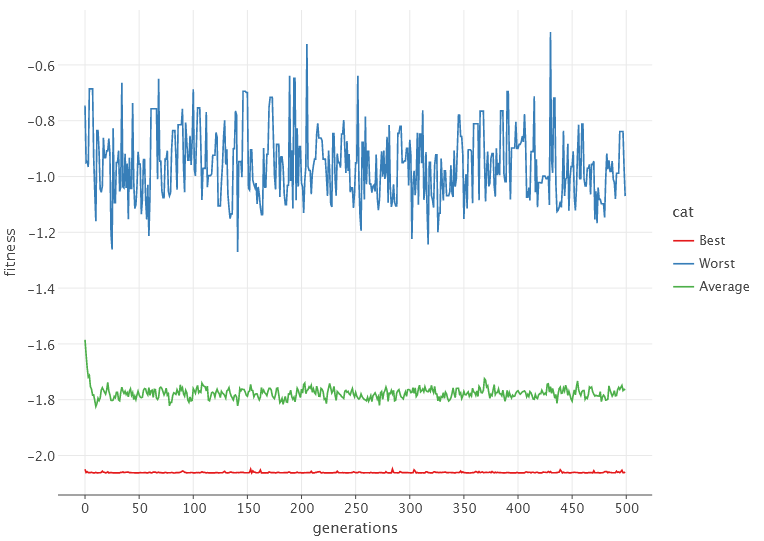
\includegraphics[width=\linewidth]{img/cross_in_tray_random.png}
      \caption{Random Selector}
    \end{subfigure}
    \begin{subfigure}{.45\textwidth}
      \centering
      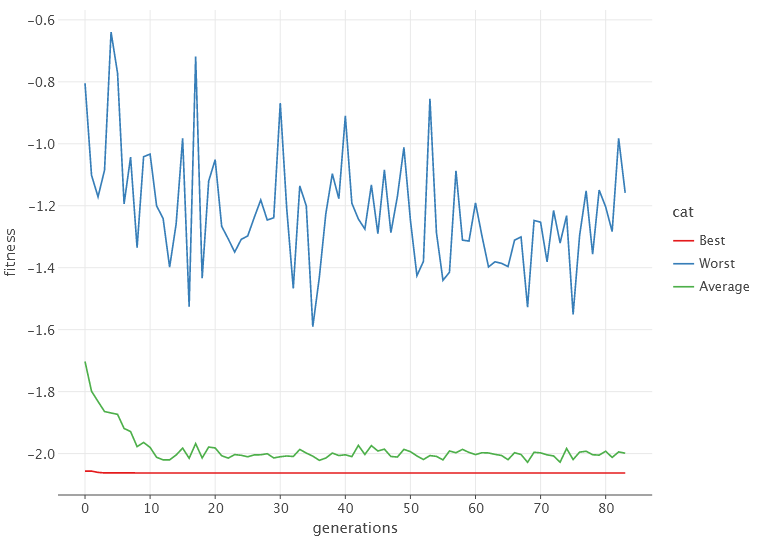
\includegraphics[width=\linewidth]{img/cross_in_tray_tournament.png}
      \caption{Tournament Selector}
    \end{subfigure}
    \begin{subfigure}{.45\textwidth}
      \centering
      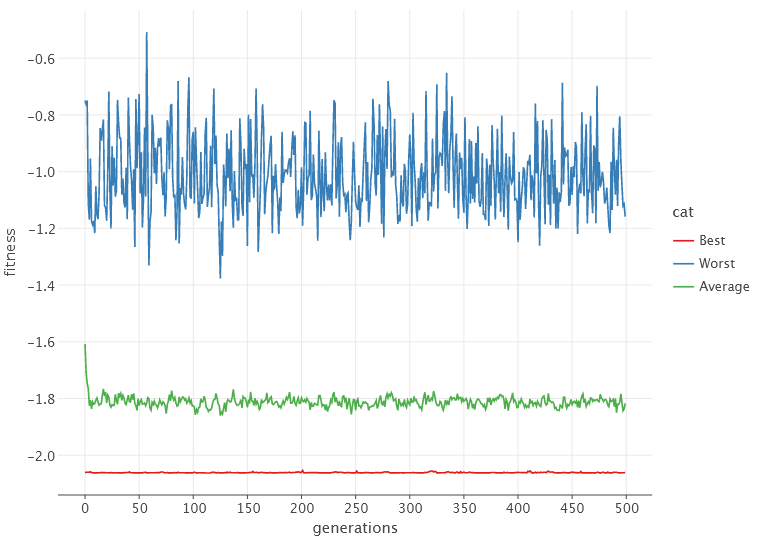
\includegraphics[width=\linewidth]{img/cross_in_tray_roulette.png}
      \caption{Roulette Selector}
    \end{subfigure}
    \caption{
      Fitness evolution for the Cross-in-tray function under different selection 
      strategies.
    }
  \end{figure}

  The comparative analysis of the selectors, as depicted in the figures, 
  highlights the superior performance of the Tournament Selector over the Random 
  and Roulette Selectors. Notably, the Random and Roulette selectors exhibit 
  comparable outcomes, which can be attributed to the inherent nature of the 
  Roulette Selector. This selector functions as a probabilistic version of the 
  Random Selector, where the selection probability is guided by individual 
  fitness weights. As the evolutionary process progresses, the variance in these 
  weights diminishes, leading to Roulette Selector's behavior increasingly 
  resembling that of the Random Selector.

  It is crucial to observe that while both Random and Roulette selectors 
  occasionally approach or even achieve the global optimum, their inherent 
  randomness impedes consistent maintenance of the optimum solution. Conversely, 
  the Tournament Selector, with its more deterministic and competitive selection 
  mechanism, not only reaches but also reliably sustains the optimal solutions 
  once discovered.

  Now we will present the results of the optimization process for each selector
  for each function.
  Each experiment was run 4 times, dropping the first iteration to avoid
  JVM warmup effects. The results presented are the average of the remaining
  3 iterations.

  \subsection{Random Selector}
      \centering
      \begin{longtable}{|l|l|l|}
        \caption{
          Time spent in each phase of the evolution process with a Random Selector.
        }\\
        \hline
        Function        & Selection (ms)        & Total (s) \\
        \hline\hline
        Ackley	          & $1.63 \times 10^{-2}$	& $7.08 \times 10^{-1}$	\\\hline
        Beale	            & $7.75 \times 10^{-3}$	& $6.05 \times 10^{-1}$	\\\hline
        Booth         	  & $5.34 \times 10^{-3}$	& $6.11 \times 10^{-1}$	\\\hline
        Bukin N.6	        & $5.69 \times 10^{-3}$	& $6.40 \times 10^{-1}$	\\\hline
        Cross-in-tray	    & $5.35 \times 10^{-3}$	& $7.24 \times 10^{-1}$	\\\hline
        Easom	            & $5.19 \times 10^{-3}$	& $6.23 \times 10^{-1}$	\\\hline
        Egg holder	      & $5.25 \times 10^{-3}$	& $5.80 \times 10^{-1}$	\\\hline
        Goldstein-Price	  & $4.90 \times 10^{-3}$	& $5.49 \times 10^{-1}$	\\\hline
        Himmelblau	      & $4.95 \times 10^{-3}$	& $5.61 \times 10^{-1}$	\\\hline
        Holder table	    & $5.24 \times 10^{-3}$	& $6.38 \times 10^{-1}$	\\\hline
        Levi	            & $5.17 \times 10^{-3}$	& $7.30 \times 10^{-1}$	\\\hline
        Matyas	          & $4.79 \times 10^{-3}$	& $5.22 \times 10^{-1}$	\\\hline
        McCormick	        & $4.41 \times 10^{-3}$	& $4.87 \times 10^{-1}$	\\\hline
        Rastrigin	        & $4.54 \times 10^{-3}$	& $5.30 \times 10^{-1}$	\\\hline
        Rosenbrock	      & $4.56 \times 10^{-3}$	& $7.79 \times 10^{-1}$	\\\hline
        Schaffer N.2	    & $4.62 \times 10^{-3}$	& $5.14 \times 10^{-1}$	\\\hline
        Schaffer N.4	    & $4.72 \times 10^{-3}$	& $5.48 \times 10^{-1}$	\\\hline
        Styblinski-Tang   & $8.03 \times 10^{-3}$	& $1.80 \times 10^{0}$	\\\hline
        Sphere	          & $5.41 \times 10^{-3}$	& $6.08 \times 10^{-1}$	\\\hline
        Three-hump camel  & $5.25 \times 10^{-3}$	& $5.70 \times 10^{-1}$	\\\hline
        \hline Average	  & $5.87 \times 10^{-3}$	& $6.67 \times 10^{-1}$ \\\hline
        S. Deviation	    & $2.56 \times 10^{-3}$	& $2.72 \times 10^{-1}$ \\\hline
      \end{longtable}

      \centering
      \begin{longtable}{|l|r|c|r|}
        \caption{Results of the optimization process with a Random Selector.}\\
        \hline
        Function  & Generations & Fittest & Error \\
        \hline\hline
        Ackley	          & $500.00$	
                          & $(0.40, -0.07)$	
                          & $4.40 \times 10^0$\\\hline
        Beale	            & $500.00$	
                          & $(-0.09, -0.29)$	
                          & $1.49 \times 10^1$\\\hline
        Booth	            & $500.0$
                          & $(0.43, 1.39)$	
                          & $3.41 \times 10^1$\\\hline
        Bukin N.6	        & $500.00$	
                          & $(-9.46, 0.70)$	
                          & $1.33 \times 10^2$\\\hline
        Cross-in-tray	    & $500.00$	
                          & $(3.24, 0.43)$	
                          & $1.91 \times 10^{-1}$\\\hline
        Easom	            & $500.0$	
                          & $(-2.91, -8.05)$	
                          & $1.00 \times 10^0$\\\hline
        Egg holder	      & $500.00$	
                          & $(-0.85, 11.64)$	
                          & $9.92 \times 10^2$\\\hline
        Goldstein-Price	  & $500.00$	
                          & $(-0.22, -0.05)$	
                          & $6.19 \times 10^2$\\\hline
        Himmelblau	      & $500.00$	
                          & $(-1.49, -2.22)$	
                          & $3.06 \times 10^2$\\\hline
        Holder table	    & $500.00$	
                          & $(0.04, 0.30)$	
                          & $1.84 \times 10^1$\\\hline
        Levi	            & $500.00$	
                          & $(0.03, 1.48)$	
                          & $8.87 \times 10^0$\\\hline
        Matyas	          & $500.00$	
                          & $(-0.92, 2.28)$	
                          & $2.75 \times 10^0$\\\hline
        McCormick	        & $500.0$	
                          & $(0.96, 0.46)$	
                          & $4.05 \times 10^0$\\\hline
        Rastrigin	        & $500.00$	
                          & $(0.42, -0.48)$	
                          & $2.42 \times 10^1$\\\hline
        Rosenbrock	      & $500.00$	
                          & $(-0.22, 0.34)$	
                          & $4.88 \times 10^1$\\\hline
        Schaffer N.2	    & $500.0$	
                          & $(7.98, -5.88)$	
                          & $7.83 \times 10^{-1}$\\\hline
        Schaffer N.4	    & $500.0$	
                          & $(-9.16, 16.31)$	
                          & $5.56 \times 10^{-1}$\\\hline
        Styblinski-Tang	  & $500.00$	
                          & $(0.50, -0.57)$	
                          & $1.91 \times 10^1$\\\hline
        Sphere	          & $500.00$	
                          & $(2.08, 0.10)$	
                          & $2.35 \times 10^{1}$\\\hline
        Three-hump camel	& $500.0$	
                          & $(-0.79, -0.78)$	
                          & $3.85 \times 10^0$\\\hline
       \hline Average	    & $500.00$	
                          & ---	
                          & $1.13 \times 10^2$\\\hline
       S. Deviation	      & $0.0$	
                          & ---	
                          & $2.48 \times 10^2$\\\hline
      \end{longtable}

  \subsection{Tournament Selector}
      \centering
      \begin{longtable}{|l|r|l|}
        \caption{
        Time spent in each phase of the evolution process with a Tournament Selector.
      }\\
        \hline
        Function          & Selection             & Total \\
        \hline\hline
        Ackley	          & $1.88 \times 10^{-1}$	& $2.08 \times 10^{-1}$	\\\hline
        Beale	            & $4.70 \times 10^{-2}$	& $2.11 \times 10^{-1}$	\\\hline
        Booth	            & $4.57 \times 10^{-2}$	& $1.80 \times 10^{-1}$	\\\hline
        Bukin N.6	        & $4.57 \times 10^{-2}$	& $2.06 \times 10^{-1}$	\\\hline
        Cross-in-tray	    & $4.42 \times 10^{-2}$	& $1.65 \times 10^{-1}$	\\\hline
        Easom	            & $4.67 \times 10^{-2}$	& $1.92 \times 10^{-1}$	\\\hline
        Egg holder	      & $4.63 \times 10^{-2}$	& $2.54 \times 10^{-1}$	\\\hline
        Goldstein-Price	  & $4.28 \times 10^{-2}$	& $1.84 \times 10^{-1}$	\\\hline
        Himmelblau	      & $4.18 \times 10^{-2}$	& $1.83 \times 10^{-1}$	\\\hline
        Holder table	    & $4.12 \times 10^{-2}$	& $2.70 \times 10^{-1}$	\\\hline
        Levi	            & $4.26 \times 10^{-2}$	& $2.00 \times 10^{-1}$	\\\hline
        Matyas	          & $4.37 \times 10^{-2}$	& $4.64 \times 10^{-1}$	\\\hline
        McCormick       	& $4.80 \times 10^{-2}$	& $1.89 \times 10^{-1}$	\\\hline
        Rastrigin	        & $4.67 \times 10^{-2}$	& $1.99 \times 10^{-1}$	\\\hline
        Rosenbrock	      & $4.84 \times 10^{-2}$	& $2.22 \times 10^{-1}$	\\\hline
        Schaffer N.2	    & $4.40 \times 10^{-2}$	& $1.77 \times 10^{-1}$	\\\hline
        Schaffer N.4	    & $4.34 \times 10^{-2}$	& $1.74 \times 10^{-1}$	\\\hline
        Styblinski-Tang	  & $4.77 \times 10^{-2}$	& $1.95 \times 10^{-1}$	\\\hline
        Sphere	          & $4.60 \times 10^{-2}$	& $4.03 \times 10^{-1}$	\\\hline
        Three-hump camel	& $4.53 \times 10^{-2}$	& $4.03 \times 10^{-1}$	\\\hline
       \hline Average	    & $5.23 \times 10^{-2}$	& $2.34 \times 10^{-1}$ \\\hline
       S. Deviation	      & $3.13 \times 10^{-2}$	& $8.39 \times 10^{-2}$ \\\hline
      \end{longtable}
      
      \label{tab:fn_opt:results:time}

      \centering
      \begin{longtable}{|l|r|c|l|}
        \caption{Results of the optimization process with a Tournament Selector.}
        \\
        \hline
        Function  & Generations & Fittest & Error \\
        \hline\hline
        Ackley	          & $115.77$	
                          & $(-6.45 \times 10^{-18}, 9.66 \times 10^{-17})$	
                          & $0.0$\\\hline
        Beale	            & $123.00$	
                          & $(2.99, 0.49)$	
                          & $5.65 \times 10^{-6}$\\\hline
        Booth	            & $116.44$	
                          & $(1.0, 3.0)$	
                          & $0.0$\\\hline
        Bukin N.6	        & $107.22$	
                          & $(-10.0, -3.51 \times 10^{-17})$	
                          & $0.0$\\\hline
        Cross-in-tray	    & $93.11$	
                          & $(-0.45, 0.44)$	
                          & $1.85 \times 10^{-6}$\\\hline
        Easom	            & $92.22$	
                          & $(3.14, 3.14)$	
                          & $0.0$\\\hline
        Egg holder	      & $172.77$	
                          & $(424.68, 463.43)$	
                          & $3.37 \times 10^1$\\\hline
        Goldstein-Price	  & $109$	
                          & $(1.70 \times 10^{-9}, -0.99)$	
                          & $7.57 \times 10^{-14}$\\\hline
        Himmelblau	      & $146.0$
                          & $(3.0, 2.0)$
                          & $0.0$\\\hline
        Holder table	    & $139.88$	
                          & $(8.05, -3.22)$	
                          & $3.59 \times 10^{-5}$\\\hline
        Levi	            & $128.77$	
                          & $(1.00, 0.99)$	
                          & $1.80 \times 10^{-25}$\\\hline
        Matyas	          & $252.11$	
                          & $(0.81, 0.32)$	
                          & $2.21 \times 10^{-1}$\\\hline
        McCormick	        & $85.88$	
                          & $(-0.54, -1.54)$	
                          & $7.70 \times 10^{-5}$\\\hline
        Rastrigin	        & $88.44$	
                          & $(1.76 \times 10^{-10}, 1.42 \times 10^{-10})$
                          & $0.0$\\\hline
        Rosenbrock	      & $137.00$	
                          & $(0.96, 0.93)$	
                          & $1.76 \times 10^{-3}$\\\hline
        Schaffer N.2	    & $87.11$	
                          & $(-5.67 \times 10^{-4}, 9.55 \times 10^{-4})$	
                          & $3.71 \times 10^{-9}$\\\hline
        Schaffer N.4	    & $98.66$	
                          & $(-3.32, -8.75)$	
                          & $3.48 \times 10^{-1}$\\\hline
        Styblinski-Tang	  & $93.11$	
                          & $(-2.90, -2.90)$	
                          & $3.91 \times 10^1$\\\hline
        Sphere	          & $383.77$	
                          & $(2.22 \times 10^{-24}, 1.52 \times 10^{-24})$	
                          & $2.19 \times 10^{-47}$\\\hline
        Three-hump camel	& $354.22$	
                          & $(4.00 \times 10^{-15}, -2.21 \times 10^{-15})$	
                          & $8.41 \times 10^{-29}$\\\hline
        \hline Average  	& $146.24$	
                          & ---	
                          & $3.67 \times 10^1$\\\hline
        S. Deviation	    & $83.23$	
                          & ---	
                          & $1.09 \times 10^1$\\\hline
      \end{longtable}

  \subsection{Roulette Selector}
      \centering
      \begin{longtable}{|l|r|r|}
        
      \caption{
        Time spent in each phase of the evolution process with a Roulette Selector.
      }
      \label{tab:fn_opt:results:time}\\
        \hline
        Function  & Selection & Total \\
        \hline\hline
       Ackley	& $0.1259916444444451$	& $0.6847722333333334$	\\\hline
       Beale	& $0.08737619999999993$	& $0.6848440666666668$	\\\hline
       Booth	& $0.07646791111111148$	& $0.5697699$	\\\hline
       Bukin N.6	& $0.08395542222222235$	& $0.6435290666666666$	\\\hline
       Cross-in-tray	& $0.0833974222222225$	& $0.6779985333333333$	\\\hline
       Easom	& $0.08038611111111091$	& $0.6832563666666666$	\\\hline
       Egg holder	& $0.0817260444444444$	& $0.7400156999999999$	\\\hline
       Goldstein-Price	& $0.08300971111111102$	& $0.6627538999999999$	\\\hline
       Himmelblau	& $0.08439613333333315$	& $0.6687351333333332$	\\\hline
       Holder table	& $0.0824499777777775$	& $0.6986748$	\\\hline
       Levi	& $0.0806594888888888$	& $0.6328013666666666$	\\\hline
       Matyas	& $0.0734033111111112$	& $0.5899227333333333$	\\\hline
       McCormick	& $0.10843388888888905$	& $0.6361473666666667$	\\\hline
       Rastrigin	& $0.07945097777777778$	& $0.6103646$	\\\hline
       Rosenbrock	& $0.0815245111111113$	& $0.5924497666666667$	\\\hline
       Schaffer N.2	& $0.07059726666666662$	& $0.5481992333333333$	\\\hline
       Schaffer N.4	& $0.06891008888888885$	& $0.5356057666666667$	\\\hline
       Styblinski-Tang	& $0.06844962222222217$	& $0.5432436333333334$	\\\hline
       Sphere	& $0.07142871111111088$	& $0.5394335$	\\\hline
       Three-hump camel	& $0.07003535555555535$	& $0.5471147$	\\\hline
      \hline Average	& $0.08210249000000003$	& $0.6244816183333333$ \\\hline
      S. Deviation	& $0.01328729027236559$	& $0.0613964541136841$ \\\hline
      \end{longtable}

      \centering
      \begin{longtable}{|l|r|r|r|}
        
        \caption{Results of the optimization process with a Roulette Selector.}
        \label{tab:fn_opt:results:roulette}\\
        \hline
        Function  & Generations & Fittest & Error \\
        \hline\hline
        Ackley	& $500.0$	& $(-0.1893911733365767, -0.34598638113431174)$	& $3.390243878441074$\\\hline
        Beale	& $500.0$	& $(-0.4871722122245125, 0.3474480357412628)$	& $22.150562167784443$\\\hline
        Booth	& $500.0$	& $(2.6869005455532124, -0.4955670499151423)$	& $60.81085149493166$\\\hline
        Bukin N.6	& $500.0$	& $(-10.284984601265123, -0.14040749281660672)$	& $6.575463259930475$\\\hline
        Cross-in-tray	& $500.0$	& $(-0.4004613371909387, -0.06692501763061005)$	& $0.11002586177693711$\\\hline
        Easom	& $500.0$	& $(3.0660500707291676, 3.2473102486188696)$	& $0.03716447878522707$\\\hline
        Egg holder	& $500.0$	& $(22.931994079832037, 40.9625899211154)$	& $848.4182927280581$\\\hline
        Goldstein-Price	& $500.0$	& $(0.08348141942073774, -0.3694022291608589)$	& $470.1256599009096$\\\hline
        Himmelblau	& $500.0$	& $(-0.7385573391672825, -1.3906357436503718)$	& $159.78255280616125$\\\hline
        Holder table	& $500.0$	& $(-3.0492234579491986, -3.074886842320195)$	& $6.274058227677354$\\\hline
        Levi	& $500.0$	& $(-0.6926610523898532, 0.23429867056177567)$	& $13.35497431109332$\\\hline
        Matyas	& $500.0$	& $(-0.016374830186079103, -0.23215662923964678)$	& $0.5066592486789856$\\\hline
        McCormick	& $500.0$	& $(1.2824940451422122, 0.7866643489405248)$	& $4.151245621384459$\\\hline
        Rastrigin	& $500.0$	& $(-1.0650002118119648, -0.7035553509112206)$	& $30.404736021622004$\\\hline
        Rosenbrock	& $500.0$	& $(-0.1515316465391131, 0.2719865942508112)$	& $6.20957198815604$\\\hline
        Schaffer N.2	& $500.0$	& $(-18.655257074502007, -8.817476416456058)$	& $0.41853389527551904$\\\hline
        Schaffer N.4	& $500.0$	& $(-15.450696513078446, 1.851760969088221)$	& $0.4686773080225914$\\\hline
        Styblinski-Tang	& $500.0$	& $(-2.7296087153895727, -2.5341893061666165)$	& $34.98094343624845$\\\hline
        Sphere	& $500.0$	& $(-0.07433850241659472, -0.6531361116341589)$	& $4.646099668177896$\\\hline
        Three-hump camel	& $500.0$	& $(0.8342425069265021, -0.48272823733652254)$	& $0.39024481167309594$\\\hline
        \hline Average	& $500.0$	& ---	& $83.66032805573943$\\\hline
        S. Deviation	& $0.0$	& ---	& $204.0917142046237$\\\hline
        \end{longtable}
